\subsection{Formula-first verification}\label{sec:res:ff}
Every analytical quantity of Sections~\ref{sec:model}--\ref{sec:theory} was
recomputed twice: from the closed forms and from independent numerical routes
(state-space to transfer-function conversion, a general CARE solver, a
frequency sweep of \eqref{eq:split} against \eqref{eq:pidf}, and an SDP solver
for \eqref{eq:lmi}). The results of Section~\ref{sec:instantiation} agree with
the values archived by the earlier version of this study, obtained with a
different code base: the gain, the poles and $\theta_0$ to all printed digits,
and the LMI bounds $\alpha_{cert}$, $\zeta_{cert}$ to within $2\times10^{-7}$
relative, the bisection tolerance. The companion MATLAB script
\texttt{cmo\_formula\_first.m} repeats the chain with \texttt{icare} and
\texttt{freqresp}.

\subsection{The equivalence, tested where it should hold and where it should fail}\label{sec:res:equiv}
Table~\ref{tab:equiv} and Fig.~\ref{fig:equiv} test Proposition~\ref{prop:struct}
on the \SI{324}{ms} reference mission with continuous-time controllers on the
nonlinear averaged plant (RK4, \SI{0.05}{\micro s}). With nominal output network
and no load pulse the LQI and its 2-DOF PIDF produce identical trajectories to
\EqNom{}, although \EqNomSat{} of the mission is spent in duty saturation, the
averaged DCM guard $i_L\ge0$ is active and the anti-windup path is exercised.
Changing $L$ by $-20\,\%$ and doubling $r_L$ and $R_{on}$ leaves the identity
intact (\EqL{}, with \EqLSat{} of saturation), exactly as the proof predicts,
because these parameters never enter the output network. The three predicted
failure modes appear with the predicted signs: a \SI{0.5}{A} load pulse
(\EqLoad{}), a \SI{+20}{\percent} load mismatch (\EqR{}) and a
\SI{+20}{\percent} capacitance mismatch that detunes $N$ from $N_C$ (\EqC{}).

Sampling is the practical case. With the zero-order-hold filter the sampled
PIDF departs from the sampled full-state LQI by \EqSampZOH{} on the
1$\to$46~V step; with the triangle-hold update \eqref{eq:foh} the departure
falls to \EqSampFOH{}, while both sampled laws sit \EqSampDelay{} from the
continuous trajectory because of the common one-sample delay. The realization is
therefore exact in continuous time and remains a close realization under
sampling \emph{provided} the filter is discretized as the capacitor-voltage
observer it is.

\begin{table}[t]
\centering
\caption{Structural-equivalence audit (Proposition~\ref{prop:struct}): largest $|v_o^{LQI}-v_o^{PIDF}|$ over the 324 ms mission.}
\label{tab:equiv}
\footnotesize
\begin{tabular}{@{}lll@{}}
\toprule
Case & predicted & measured\\
\midrule
nominal, $i_p=0$ & identical & \EqNom\\
$L-20\,\%$, $r_L\times2$, $R_{on}\times2$ & identical & \EqL\\
0.5 A load pulse & $\ne$, Eq.~\eqref{eq:gap} & \EqLoad\\
$R+20\,\%$ & $\ne$, Eq.~\eqref{eq:gap} & \EqR\\
$C+20\,\%$ & $\ne$, $N\neq N_C$ & \EqC\\
sampled, ZOH filter, 1$\to$46 V & close & \EqSampZOH\\
sampled, FOH filter \eqref{eq:foh}, 1$\to$46 V & close & \EqSampFOH\\
\bottomrule
\end{tabular}
\end{table}

\begin{figure}[t]
\centering
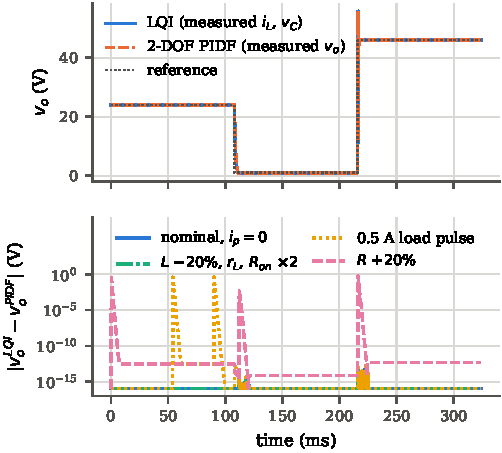
\includegraphics[width=\columnwidth]{figures/fig_equivalence.pdf}
\caption{Top: LQI with measured $(i_L,v_C)$ and its 2-DOF PIDF with measured $v_o$ on the reference mission (continuous time, averaged nonlinear plant, saturation active). Bottom: absolute output difference; the nominal and inductor-branch-mismatch curves lie at the floating-point floor, the load-pulse and load-mismatch curves show the predicted departures.}
\label{fig:equiv}
\end{figure}
